\documentclass[25pt, a0paper, portrait, innermargin=0.5cm, margin=0cm, colspace=0.5cm, blockverticalspace=8mm]{tikzposter}

\usepackage{fontspec}        % Allows font customization
\usepackage[T1]{fontenc}     % Use T1 font encoding

\setmainfont{Ubuntu}  % Set the main text font
\setsansfont{Ubuntu}            % Set the sans-serif font
\setmonofont{Ubuntu Mono}      % Set the monospaced font

\usepackage[backend=bibtex, style=numeric, sorting=none, locallabelwidth]{biblatex}
\bibliography{refs}

\usepackage{wrapfig}
\usepackage{authblk}

\title{Low Cost Silicon-based Semiconductor Device Manufacturing}

% Define colors (optional)
\definecolor{titlebgcolor}{RGB}{0,120,180}
\definecolor{blocktitlebgcolor}{RGB}{180,180,180}
\definecolor{blockbgcolor}{RGB}{240,240,240}

% Custom styles
\usetheme{Autumn}
\usecolorstyle{Default}

\renewcommand\Affilfont{\LARGE}
\renewcommand{\Authfont}{\LARGE}

\author[1]{Patryk Wlazłyń}
\author[2]{Rafał Mikołajczyk}
\author[2]{Kornel Uriasz}
\author[2]{Maciej Pacholczyk}
\affil[1]{Independent, Wrocław, Poland}
\affil[2]{Politechnika Wrocławska, Wybrzeże Stanisława Wyspiańskiego 27, 50-370 Wrocław}

\makeatletter
\def\maketitle{\AB@maketitle}
\makeatother

\begin{document}

\maketitle

%%
%% A bit hacky way of inserting images in the title bar, but it works.
%% Recommended by the author of tikzposter https://tex.stackexchange.com/a/489933
%%

% Upper left corner, QR for holzcoredump.cc/pubs/jaszowiec2024/poster.pdf
\node[anchor=west, yshift=0.5cm] at (TP@title.west) {
\includegraphics[width=10cm]{qrcode_poster.png}};
\node[anchor=west, xshift=2cm, yshift=-4.75cm] at (TP@title.west) {\LARGE POSTER};

% Upper right corner, QR for holzcoredump.cc/pubs/jaszowiec2024/paper
\node[anchor=east, yshift=0.5cm] at (TP@title.east) {
\includegraphics[width=10cm]{qrcode.png}};
\node[anchor=east, xshift=-0.9cm, yshift=-4.75cm] at (TP@title.east) {\LARGE MORE INFO};

\begin{columns}
    \column{1,00}
    \block{Motive}{
        High costs of acquiring and maintaining specialized and high quality
        equipment for semiconductor manufacturing poses a challenge for
        individuals to experiment and learn about the technology.  \textbf{We
        present cost-effective methods for engineering equipment and complete
        process for silicon-based semiconductor device manufacturing and
        testing.} We focused on obtaining results in an easily affordable
        environments by sacrificing economic scaling and quality of the
        manufactured devices.  \textbf{We aim to pave the way for students and
        enthusiasts interested in semiconductor manufacturing.}
    }
\end{columns}

\begin{columns}
    \column{0.50}
    \block{High temperature furnace}{
        Electric furnace that can reach up to \textbf{1200°C}. It is used for
        \textbf{oxide growth} and \textbf{diffusion doping}. It is built using
        the firebricks and resistance wire, \textbf{wirelessly controlled}
        using Raspberry Pi Pico W microcontroller\cite{picow}. The temperature
        is measured with pt100 temperature sensor. It has a \textbf{water pump}
        mounted at the top with the quartz tube going
        inside the furnace, allowing \textbf{wet oxidation} of the wafers. Type
        K thermocouple is used to measure the temperature inside the furnace.
        The microcontroller can control the rate of heating, automatic
        temperature steering and water pumping.  We provide an \textbf{open
        source firmware and PCB design}\cite{firmware}.
        \begin{tikzfigure}
            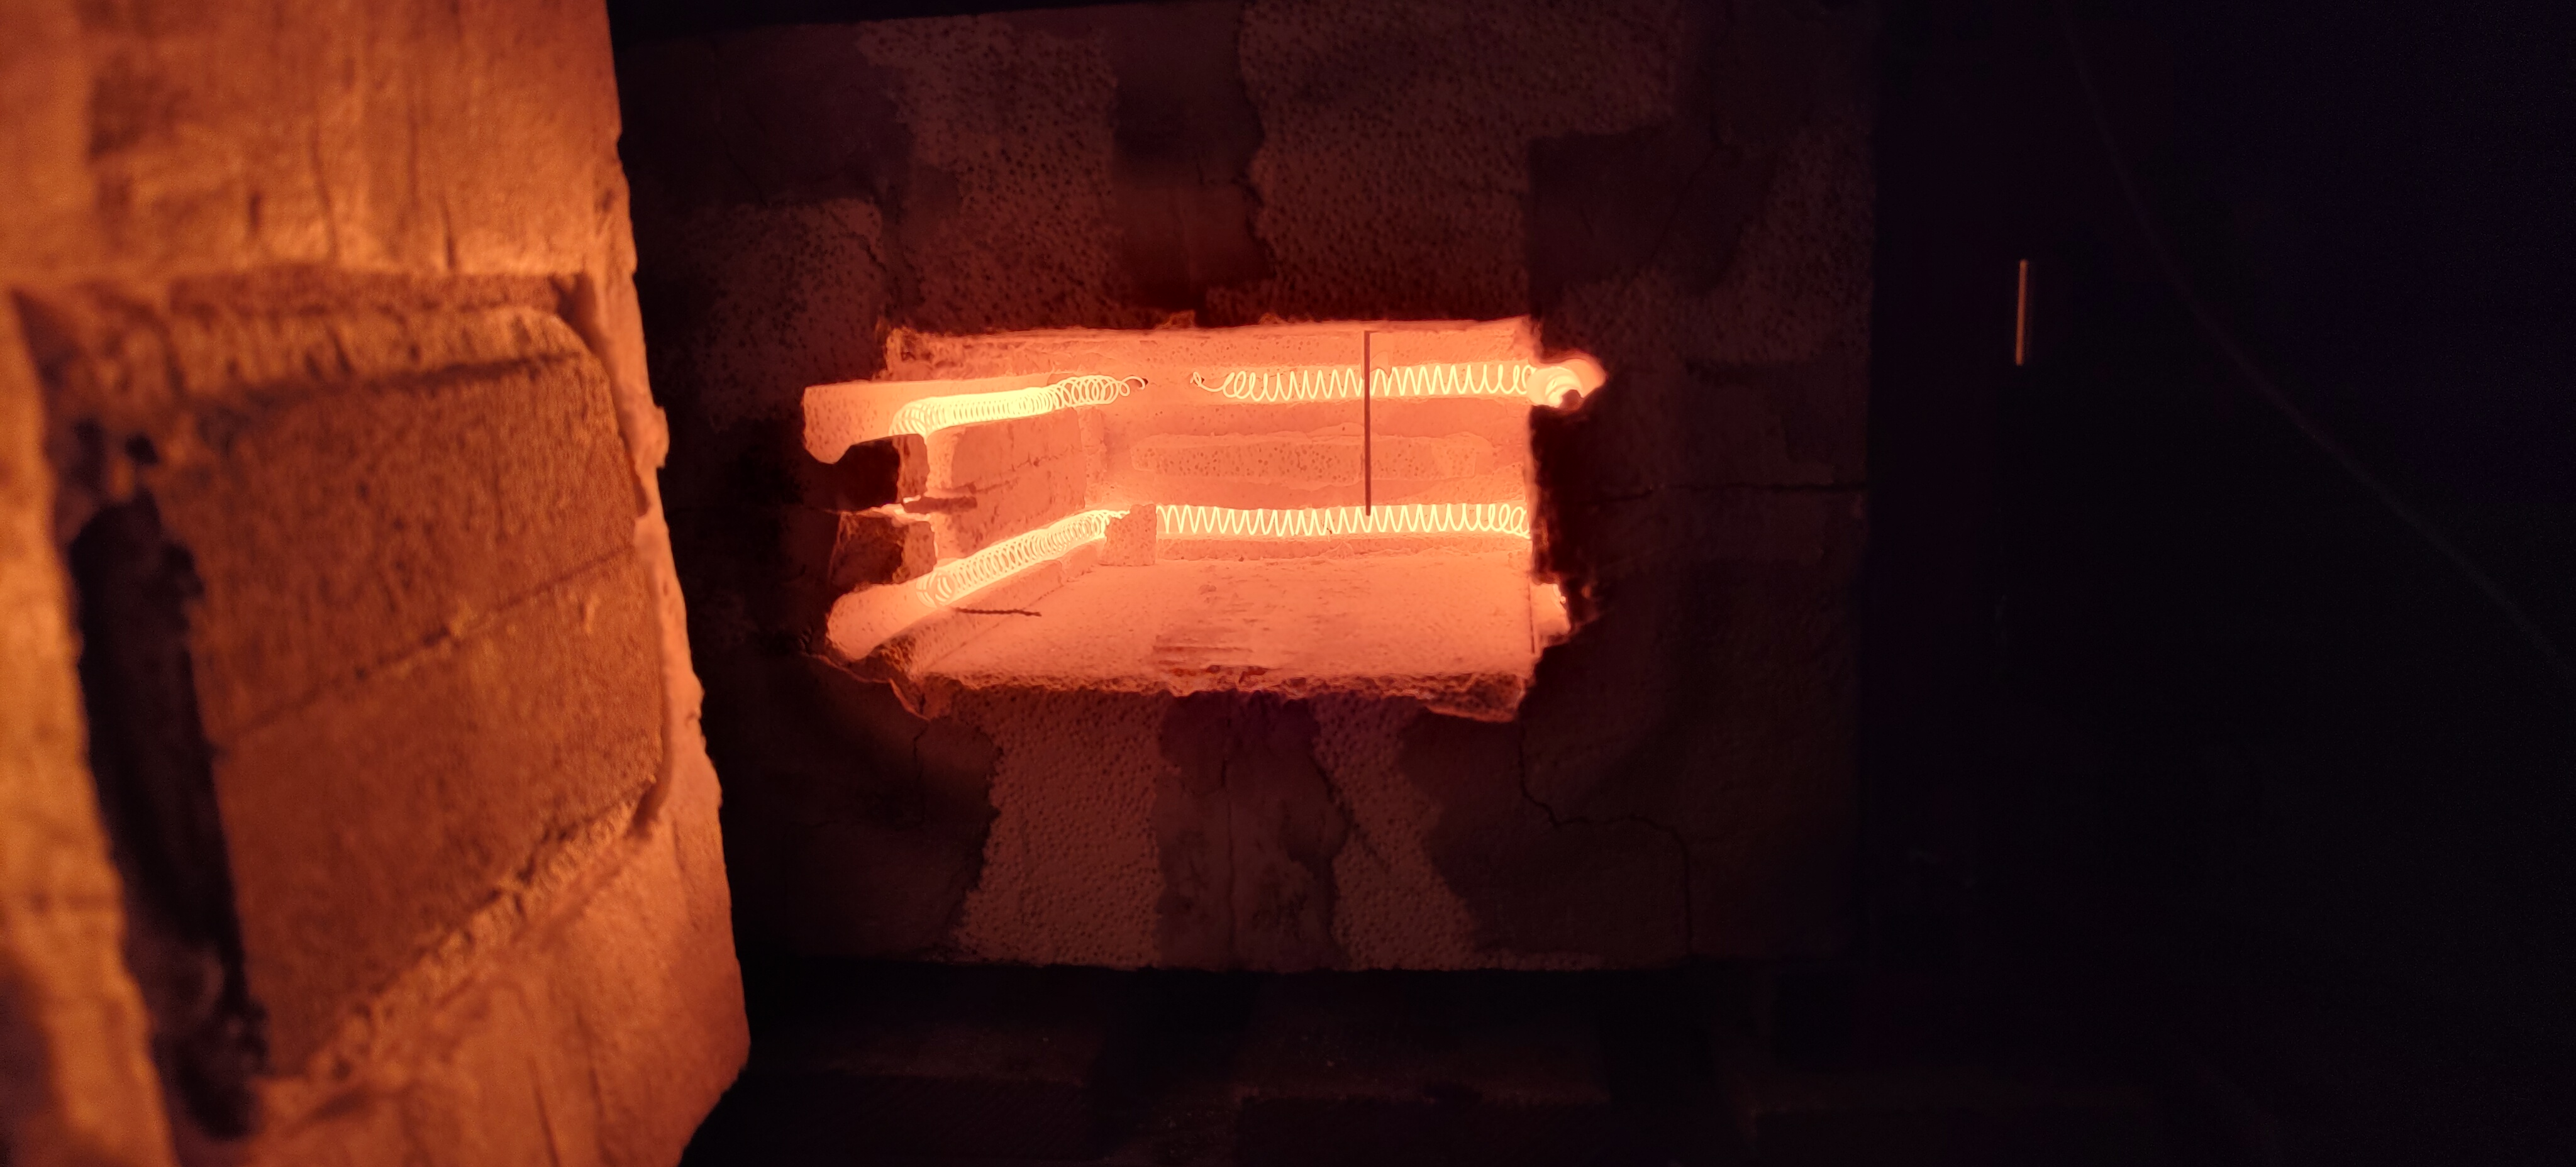
\includegraphics[width=0.45\textwidth]{media/furnace_2.jpg}
        \end{tikzfigure}
    }

    \block{Photolithography}{
        We do \textbf{maskless photolithography}, using \textbf{DLP projector}
        with the \textbf{modified optics} to obtain a sharp image on the
        surface of the wafer. We pattern the wafer using \textbf{AZ 1512 HS
        photoresist}\cite{az1512} with \textbf{AZ 351 B developer}\cite{az351b}
        from MicroChemicals, spin coated on top of it. The projector is mounted
        vertically, aiming at the flat bed underneath where the wafer is
        positioned.  Desired \textbf{pattern is prepared in JPEG format} using
        GIMP\cite{gimp} and displayed with the DLP using a PC. DLP projectors
        are based on \textbf{mercury vapor lamp}, which emit UV light and
        \textbf{DMD (digital micromirror device) chip}\cite{dlp}. We use
        combination of white and black pixels in the image to select which part
        of the wafer should be exposed to UV. There is a 3D-printed shutter
        connected to the electric motor driven by Raspberry Pi Pico
        W\cite{picow}, which can be used to expose the wafer for the desired
        duration, controlling the amount of UV that hits the photoresist.  We
        provide the microcontroller \textbf{firmware as an open source
        software}\cite{firmware}.
        \begin{tikzfigure}
            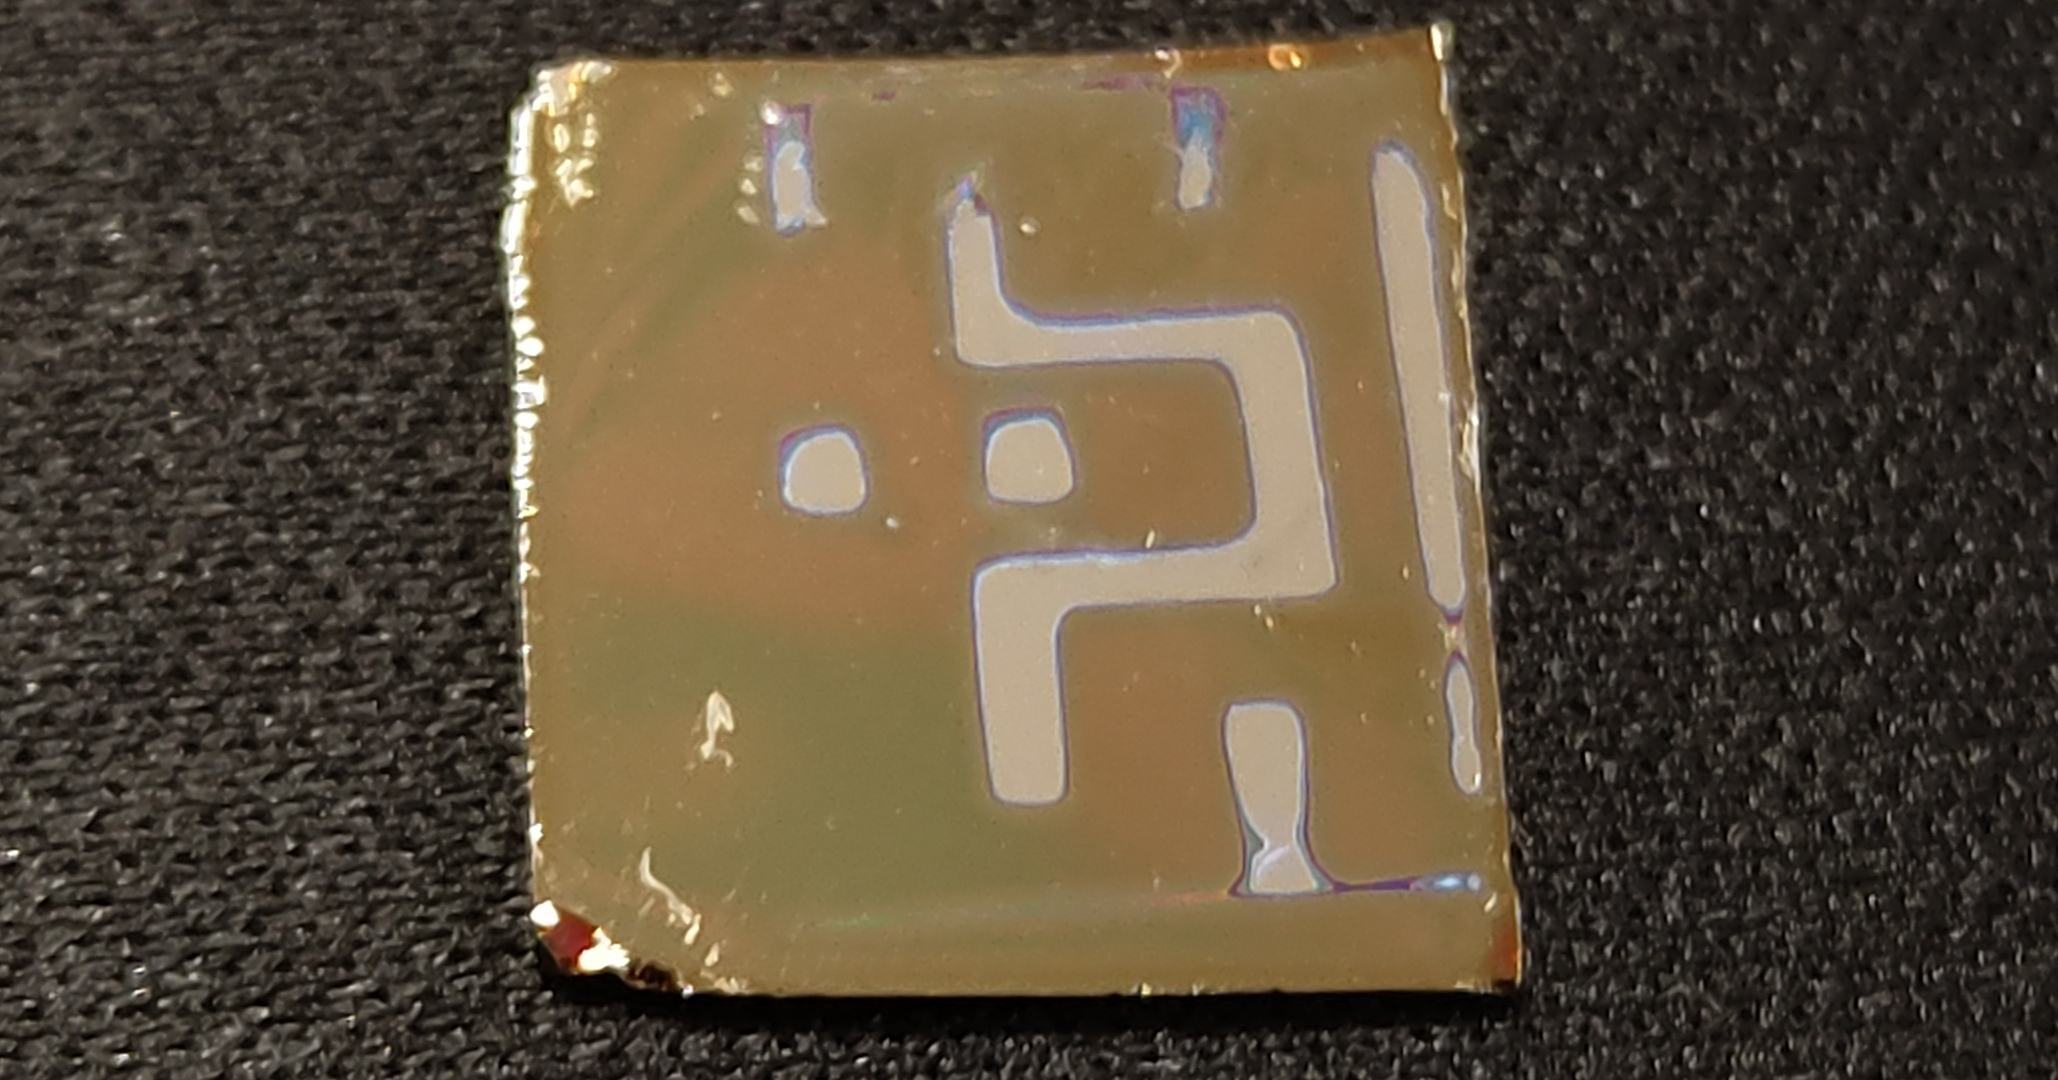
\includegraphics[width=0.45\textwidth,height=0.15\textwidth]{media/pl_background.jpg}
        \end{tikzfigure}
    }

    \block{Contacts}{
        Contacts are done using silver epoxy and copper wires. The other end of
        the wire can then make a direct contact with the probe or soldered into
        a prototyping board or PCB for testing.
    }

    \column{0.50}
    \block{Hotplate}{
        \begin{wrapfigure}{r}{0.2\textwidth}
            \begin{tikzfigure}
                \includegraphics[width=400pt]{media/hotplate_noplate.jpg}
            \end{tikzfigure}
        \end{wrapfigure}
        Electric hotplate that can reach up to \textbf{400°C}. Based on the
        firebricks and resistance wire. Used for soft and post-exposure bake of
        photoresist, synthesis of tetraethyl orthosilicate based Spin-On-Dopant
        and it's predeposition step before diffusion doping in the furnace.
        Raspberry Pi Pico W microcontroller\cite{picow} is used for wireless
        access, controlling rate of heating and automatic temperature steering.
        We provide the microcontroller \textbf{firmware as an open source
        software}\cite{firmware}.
    }

    \block{Doping}{
        \textbf{We propose a modified process to the one described in Fangsuwannarak et
        Al. 2019 \cite{Fangsuwannarak}}. It yields a less, but sufficiently viscous
        dopant and significantly \textbf{extends its shelf life at room temperature}.
        We spin coat the dopant on the wafer, do pre deposition on hot plate
        and thermal diffusion in the furnace. This creates
        N-doped wells and phosphosilicate glass (PSG). The PSG is stripped
        using \( NH_{4}F\cdot HF\) solution dissolved in DI water.
        For \textbf{selective doping}, we use thick (\(\sim\)500nm) thermally grown
        \(SiO_{2}\), that stops spin coated SOD from penetrating too far into
        the wafer.
        We control for rate of doping by doing a \textbf{double-oxidation}
        process, which grows two layers of \(SiO_{2}\), one, for completely
        stopping the doping \(\sim\)500nm and another in a range of 30-100nm,
        which acts as a doping limiter and not a complete stopper.
    }

    \block{Spin coating}{
        We successfully used a 3000 RPM, 12V \textbf{computer fan} to
        manufacture solar cells and NPN MOSFET devices with a double-sided tape
        on which the wafer is placed. The solution, while very cheap and
        simple, but is not very convenient. The tape has to be replaced
        frequently, and contaminates the back of the wafer. For this reason, we
        \textbf{designed and 3D-printed} a \textbf{rotating bed} with an
        opening in the middle and a chamber.  The bed is connected to the
        \textbf{BLDC motor} that can spin the bed to up to \textbf{4000 RPM}.
        We use \textbf{infrared light source and detector}, connected to the
        Raspberry Pi Pico microcontroller\cite{picow}, forming a
        \textbf{feedback} and allowing us to \textbf{control the rotating speed
        of the bed}. The opening in the bed is connected through a hose to the
        modified \textbf{vacuum cleaner} that sucks the wafer down to the bed.
    }

    \block{References}{
        \nocite{*}
        \printbibliography[heading=none]
    }
\end{columns}

\begin{columns}
    \column{1.00}
    \block{Testing \& results}{
        We were able to make various devices, including \textbf{resistors},
        \textbf{solar cells}, \textbf{capacitors} and \textbf{MOSFETs}. \\
        It's important to note, that the obtained results are
        \textbf{significantly worse than their commercial equivalents} and that
        they are \textbf{primarily useable as a learning ground and
        experimentation}, with the main advantage of relatively \textbf{easy
        access} to the required tooling and components used to build the whole
        lab.
    }
\end{columns}

\begin{columns}
    \column{0.50}
\end{columns}

\end{document}